\section{Matched-Resource Controls: What Is the Confidence Statistic
Actually Buying?}
\label{sec:matched}

Every module works by spending more than baseline, which raises the
strongest objection available against this paper and one the ablation of
Sec.~\ref{sec:results} cannot answer: perhaps the gains have nothing to
do with confidence guidance, and any comparable budget increase ---
however allocated --- would do as well. Stage 3 tests exactly this, giving
the Baseline code path each adaptive arm's own realised budget spread
uniformly, with no confidence computation anywhere in the control
(Table~\ref{tab:matched}, Fig.~\ref{fig:matched}).

\textbf{No individual module is distinguishable from its matched
control.} Module B and its candidates-matched control both succeed on
77.1\% of trials, differing on two trials in opposite directions
($b{=}1$, $c{=}1$, $p=1.00$). Module C and its beam-matched control agree
on every single trial ($b{=}c{=}0$, $p=1.00$). Module D reaches 76.4\%
against its control's 73.6\% --- $+2.8$ pp with an interval spanning zero
($[-6.9,+11.8]$, $b{=}22$, $c{=}26$, $p=0.67$), 48 discordant trials
split almost evenly. None comes close to surviving Holm correction
(\SItables{}).

\textbf{The combination is distinguishable.} Full reaches 100\% against
the shots-matched control's 73.6\%: $+26.4$ pp (95\% CI $[+19.4,+33.3]$),
fixing 38 trials the control failed and breaking none ($b{=}0$, $c{=}38$,
$p=7.3\times10^{-12}$). This is the weaker of the two directions the
comparison could have been run in, since the control was matched on shots
alone while Full also widened candidates and beam --- a caveat we return
to below.

\paragraph{What this licenses us to claim, and what it does not.} It does
not license the claim that placing budget by confidence beats placing the
same budget uniformly: at the instance sizes we can reach it does not,
and we found no evidence that it does. What the controls establish is
narrower --- the statistic \emph{recovers} a budget as good as an
oracle-matched uniform one \emph{without being told what that budget
is}. The controls are not algorithms anyone could run: each is built from
diagnostics recorded while watching the adaptive rule make its choices on
that very trial. Sec.~\ref{sec:discussion} develops what this does and
does not support.

There is a second, quantitative reading. The budgets the controls were
handed are large --- a mean of $43.7$ extra shots per window on a grid
whose starved settings are 4--16, a matched candidate count of $4.29$
against a baseline $k\in\{1,2\}$, a matched beam width of $21.1$ against
$P\in\{1,2\}$ (\SItables{}) --- and the adaptive rules arrived at these
multiples from the counts alone. That the uniform version of the same
total performs equally well is a statement about \emph{this} regime: few
windows, small orders, and ambiguity spread fairly evenly across windows.
We would expect the two to separate where ambiguity is concentrated in a
minority of windows, but we have no instance in reach that exhibits that
concentration, so we do not claim it.

\paragraph{How exact is the matching?} The beam-matched control is
exact: $P'$ is already a trial-level scalar, and the control receives
that trial's value unchanged, so its realised beam width equals module
C's on every trial. The other two approximate a non-uniform per-window
allocation by its mean, and the direction of the residual error matters,
so we report it. The candidates-matched control received a mean
$k=4.29$ against module B's mean realised $m_w=4.25$: it was, if
anything, \emph{over}-matched, which makes B's null result harder rather
than easier to obtain. The shots-matched control received a mean of
$43.70$ extra shots per window against the $43.82$ module D actually
drew --- under-matched by $0.3\%$, a shortfall far too small to account
for D's $+2.8$~pp point estimate, and in the direction that favours D.
Neither residual changes the conclusion.

\paragraph{The remaining limit of the controls.} Matching a non-uniform
allocation by its mean is the natural uniform counterpart, but it is not
the only possible one, and a differently-constructed control could
behave differently. More importantly, \textbf{no control matches all
three budgets simultaneously against the Full arm}. The
Full-vs-control comparison equalises shots only, so its $+26.4$~pp
cannot be attributed to confidence guidance alone --- part of it is
simply the candidate and beam budget that the control never received.
Constructing a fully matched three-way control is a direct extension of
the released instrumentation and is the single experiment we would add
next; we flag its absence rather than let the $p=7.3\times10^{-12}$
stand unqualified.

\begin{table}[htbp]
\centering\small
\caption{Matched-resource controls on the canonical 144-trial grid. Each
control runs the Baseline code path, with all module flags disabled, at
the uniform budget derived from that trial's own adaptive diagnostics.
$b$ = trials where the control succeeded and the adaptive arm failed;
$c$ = the reverse. The upper block is the reference gain over an
unmodified baseline; the lower block is the comparison that matters.}
\label{tab:matched}
\resizebox{\linewidth}{!}{%
\begin{tabular}{@{}lccccc@{}}
\toprule
Comparison & Reference & Arm & Diff.\ [95\% CI] & $(b,c)$ & Exact $p$ \\
\midrule
\multicolumn{6}{@{}l}{\emph{Controls do improve on an unmodified baseline}}\\
candidates-matched vs.\ Baseline & 52.1\% & 77.1\% & $+25.0$ pp $[+18.1,+33.3]$ & $(2,38)$ & $1.5\times10^{-9}$ \\
beam-matched vs.\ Baseline       & 52.1\% & 56.9\% & $\phantom{0}+4.9$ pp $[+1.4,+8.3]$ & $(0,7)$ & $1.6\times10^{-2}$ \\
shots-matched vs.\ Baseline      & 52.1\% & 73.6\% & $+21.5$ pp $[+11.8,+31.3]$ & $(13,44)$ & $4.7\times10^{-5}$ \\
\midrule
\multicolumn{6}{@{}l}{\emph{Adaptive arm vs.\ its own matched control}}\\
B vs.\ candidates-matched & 77.1\% & 77.1\% & $\phantom{0}+0.0$ pp $[-2.1,+2.1]$ & $(1,1)$ & $1.00$ \\
C vs.\ beam-matched       & 56.9\% & 56.9\% & $\phantom{0}+0.0$ pp $[+0.0,+0.0]$ & $(0,0)$ & $1.00$ \\
D vs.\ shots-matched      & 73.6\% & 76.4\% & $\phantom{0}+2.8$ pp $[-6.9,+11.8]$ & $(22,26)$ & $0.67$ \\
\textbf{Full vs.\ shots-matched} & \textbf{73.6\%} & \textbf{100.0\%} & $\mathbf{+26.4}$ \textbf{pp} $[+19.4,+33.3]$ & $(0,38)$ & $7.3\times10^{-12}$ \\
\bottomrule
\end{tabular}
}
\end{table}

\begin{figure}[htbp]
\centering
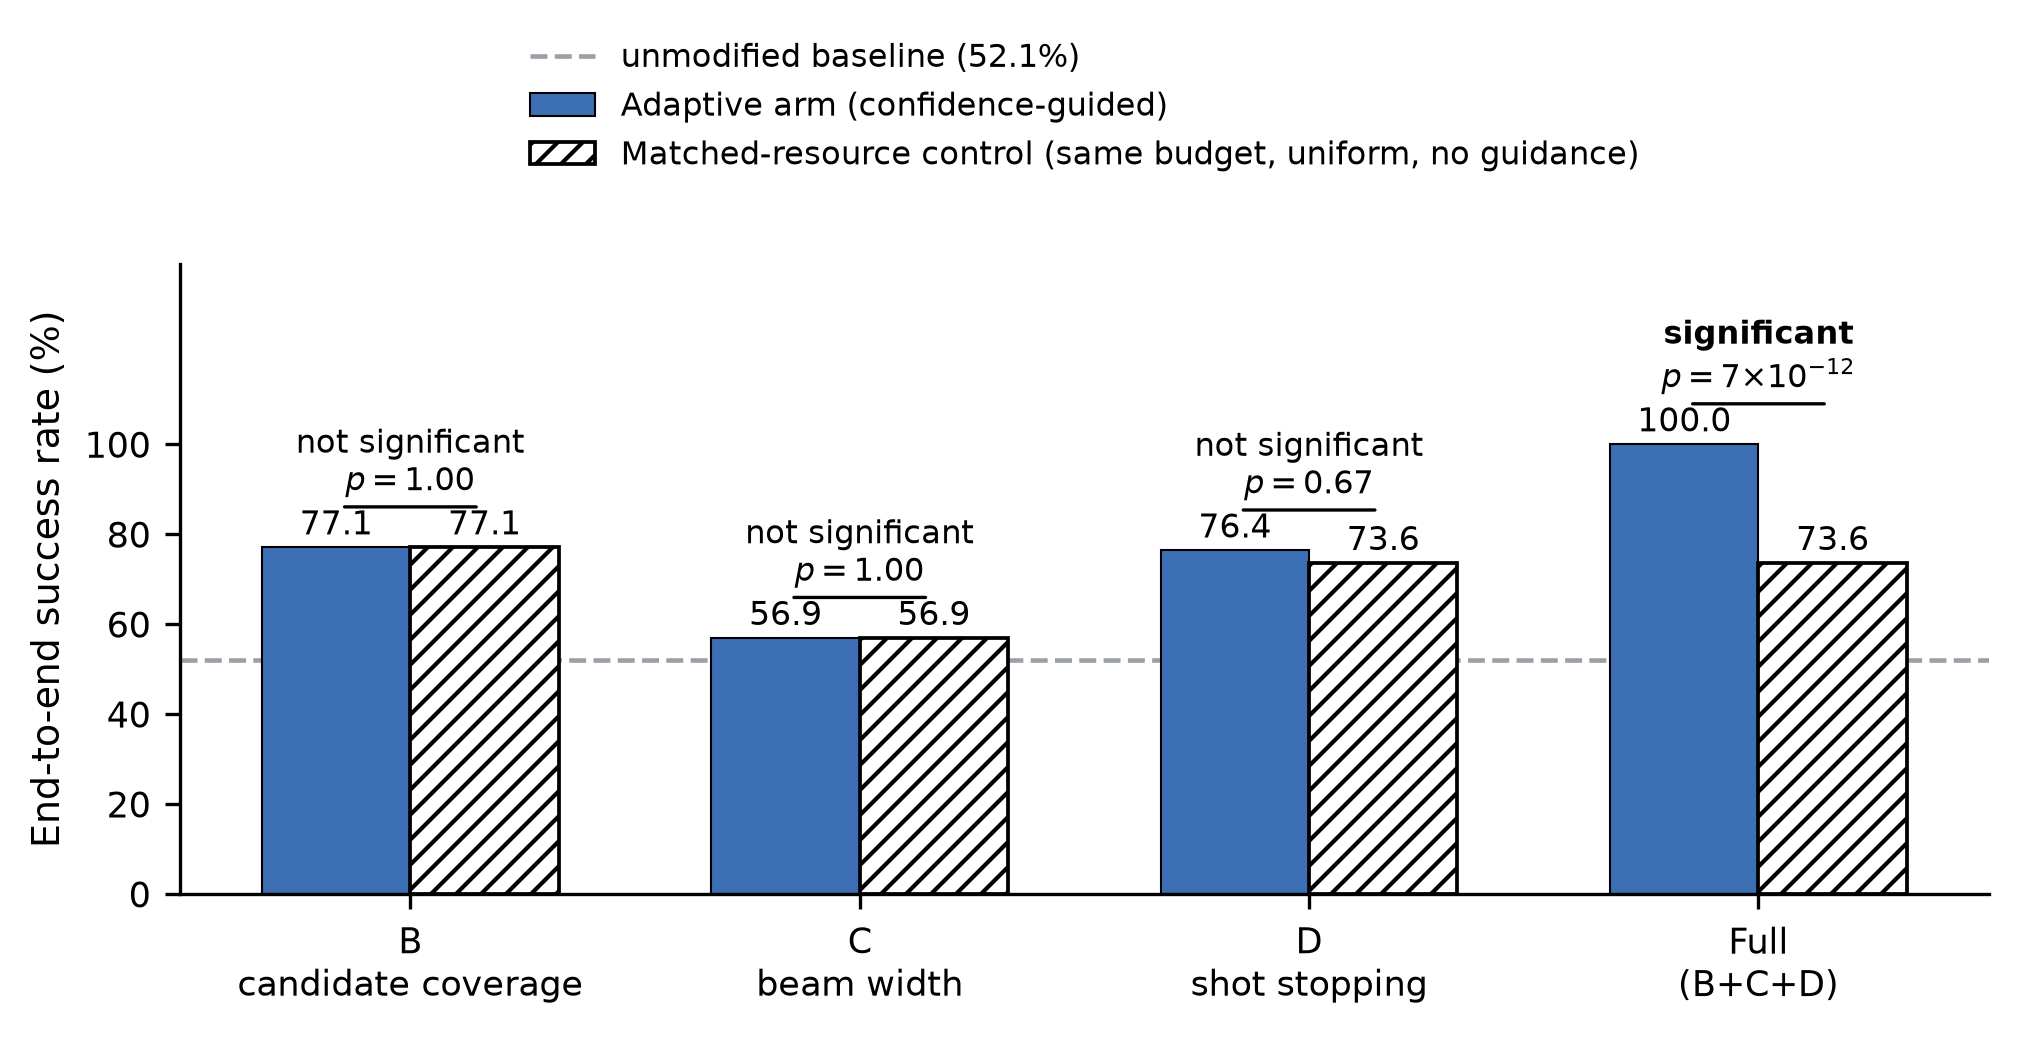
\includegraphics[width=0.94\linewidth]{../Data/failure_study/plots/paper_fig4_matched_resource.png}
\caption{\textbf{Is the gain due to confidence guidance, or to the size
of the budget it requests?} Each adaptive arm beside a control run
through the baseline code path at that arm's \emph{own} realised budget,
spread uniformly, with no confidence computation anywhere. Canonical
grid, 144 seed-paired trials. \textbf{The central result is the three
``not significant'' labels}: taken one at a time, none of the modules
outperforms an equally-resourced uniform allocation. Only the full
combination separates from its control, and that control is matched on
shots alone (Limitation~2). The controls are oracles,
not competitors --- their budgets could only be known after watching the
adaptive rule choose them. Rendered from
\texttt{phase7\_matched\_resource.csv}.}
\label{fig:matched}
\end{figure}
